\documentclass[11pt]{article}
\usepackage[utf8]{inputenc}
\usepackage[T1]{fontenc}
\usepackage[margin=1in]{geometry}
\usepackage{amsmath,amssymb,amsthm}
\usepackage{booktabs}
\usepackage{array}
\usepackage{url}
\usepackage{microtype}
\usepackage{graphicx}
\usepackage{caption}
\usepackage{xcolor}
\usepackage{listings}
\usepackage[hidelinks]{hyperref}
\makeatletter\g@addto@macro{\UrlBreaks}{\do\_\do\.\do\/}\makeatother
\emergencystretch=3em
\tolerance=2000
% generated by gen_inputs.py -- do not edit
\newcommand{\PHKstar}{3.00379}
\newcommand{\PHKstarLo}{3.0025}
\newcommand{\PHKstarHi}{3.0051}
\newcommand{\PHTwoKstar}{6.008}
\newcommand{\PHhbarc}{1.5685}
\newcommand{\PHhbarTwoM}{0.52218}
\newcommand{\PHNPoints}{99}
\newcommand{\PHNXray}{49}
\newcommand{\PHNNeutron}{50}
\newcommand{\PHNCons}{29}
\newcommand{\PHNUnd}{7}
\newcommand{\PHNRef}{63}
\newcommand{\PHNRefXray}{32}
\newcommand{\PHNRefNeutron}{31}
\newcommand{\PHDeltaDS}{0.082}
\newcommand{\PHPeakX}{1.458}
\newcommand{\PHPeakXQ}{2.058}
\newcommand{\PHPeakN}{1.376}
\newcommand{\PHPeakNQ}{2.070}
\newcommand{\PHRmsSpline}{0.019}
\newcommand{\PHLastConsQ}{1.400}
\newcommand{\PHLastConsS}{0.464}
\newcommand{\PHLastConsB}{0.483}
\newcommand{\PHFirstExQ}{1.470}
\newcommand{\PHFirstExS}{0.532}
\newcommand{\PHFirstExB}{0.495}
\newcommand{\PHStrictLo}{1.550}
\newcommand{\PHStrictHi}{5.129}
\newcommand{\PHNominalHi}{5.94}
\newcommand{\PHRotonN}{21}
\newcommand{\PHRotonRatioLo}{1.62}
\newcommand{\PHRotonRatioHi}{2.49}
\newcommand{\PHRotonMinMargin}{0.328}
\newcommand{\PHPeakBound}{0.585}
\newcommand{\PHPeakS}{1.458}
\newcommand{\PHPeakQ}{2.058}
\newcommand{\PHCtlBogViol}{0}
\newcommand{\PHCtlBogN}{99}
\newcommand{\PHCtlBogMax}{0.9999996}
\newcommand{\PHFpOne}{0}
\newcommand{\PHFpTwo}{0.0005}
\newcommand{\PHFpFour}{0.41}
\newcommand{\PHCtlFreeNom}{95}
\newcommand{\PHCtlFreeStrict}{89}
\newcommand{\PHCtlPlantNom}{89}
\newcommand{\PHCtlPlantStrict}{81}
\newcommand{\PHParseA}{300}
\newcommand{\PHParseB}{266}
\newcommand{\PHFeynN}{68}
\newcommand{\PHFeynExceed}{2}
\newcommand{\PHFeynQa}{0.213}
\newcommand{\PHFeynQb}{0.267}
\newcommand{\PBPeakFail}{16}
\newcommand{\PBMeanFail}{4}
\newcommand{\PBCeffFail}{8}
\newcommand{\PBLdaFail}{0}
\newcommand{\PBNCurve}{24}
\newcommand{\PBSolidMax}{0.0022}
\newcommand{\PBClosedA}{1.0e-06}
\newcommand{\PBClosedB}{9.9e-05}
\newcommand{\PBQ}{2.506}
\newcommand{\PBGridViol}{0}
\newcommand{\PBGridN}{42}
\newcommand{\PBGridFree}{38}
\newcommand{\PBSkRatioLo}{0.82}
\newcommand{\PBSkRatioHi}{0.95}
\newcommand{\PBSkBoundLo}{0.44}
\newcommand{\PBSkBoundHi}{0.58}
\newcommand{\PBStN}{13}
\newcommand{\PBStNominal}{3}
\newcommand{\PBStOne}{0}
\newcommand{\PBStRaw}{0}
\newcommand{\PBStMaxZ}{0.31}
\newcommand{\PBStOpenRms}{0.026}
\newcommand{\PBStOpenMax}{0.059}
\newcommand{\PLNBasic}{21}
\newcommand{\PLNNeg}{4}
\newcommand{\PLNPos}{3}
\newcommand{\PLGate}{PASS}
\newcommand{\PLSecBasic}{10.5}
\newcommand{\PLRcBasic}{0}
\newcommand{\PLSecNeg}{6.9}
\newcommand{\PLRcNeg}{0}
\newcommand{\PLSecPos}{6.7}
\newcommand{\PLRcPos}{0}
\newcommand{\PLSecCtl}{6.2}
\newcommand{\PLRcCtl}{0}
\newcommand{\PLShaBasic}{a8ed4357bce846e675af161a81dbeddeedcba07c0a2e7f2ae09fce21c5cb6432}
\newcommand{\PLShaShortBasic}{a8ed4357bce8}
\newcommand{\PLLinesBasic}{353}
\newcommand{\PLShaNeg}{182f8135dd3c778703a8523e46724f600227a3bdcaadc4da5a8bc843373bfc3a}
\newcommand{\PLShaShortNeg}{182f8135dd3c}
\newcommand{\PLLinesNeg}{81}
\newcommand{\PLShaPos}{1555d75cda679a600b667ac0f559b7bd72f9cee3982c644531ee6f81d4bffc05}
\newcommand{\PLShaShortPos}{1555d75cda67}
\newcommand{\PLLinesPos}{93}
\newcommand{\PLShaCtl}{a0f2e8edab9b5aa211fd1a5b39d8836cc22220b483390413edda46135e0c0099}
\newcommand{\PLShaShortCtl}{a0f2e8edab9b}
\newcommand{\PLLinesCtl}{33}
\newcommand{\PLShaMatch}{match}
\newcommand{\PLRerun}{reproduced the same rc and axiom lines}
\newcommand{\PLReSecBasic}{12.4}
\newcommand{\PLReRcBasic}{0}
\newcommand{\PLReSecNeg}{8.4}
\newcommand{\PLReRcNeg}{0}
\newcommand{\PLReSecPos}{7.5}
\newcommand{\PLReRcPos}{0}
\newcommand{\PLReSecCtl}{6.1}
\newcommand{\PLReRcCtl}{0}
\newcommand{\PXPosOne}{1.7e-15}
\newcommand{\PXPosTwo}{6.7e-16}
\newcommand{\PXPosTrial}{1.1e-16}
\newcommand{\PXSector}{200\slash 200}
\newcommand{\PXPosBog}{1.8e-16}
\newcommand{\PXHeight}{2000\slash 2000}
\newcommand{\PXNegMin}{0.0019}
\newcommand{\PXNegMed}{0.079}
\newcommand{\PXNegCaught}{200\slash 200}
\newcommand{\PLedN}{31}
\newcommand{\PLedA}{11}
\newcommand{\PLedL}{5}
\newcommand{\PLedC}{7}
\newcommand{\PLedX}{8}
\newcommand{\PGateExit}{1}
\newcommand{\PGateBlock}{0}
\newcommand{\PGateFlag}{11}

\lstset{basicstyle=\ttfamily\scriptsize,columns=fullflexible,keepspaces=true,breaklines=true,
  frame=single,framesep=2pt,xleftmargin=3pt,xrightmargin=3pt,upquote=true,
  keywordstyle=\bfseries,morekeywords={theorem,lemma,def,noncomputable,abbrev,where,fun,Prop,axiom},
  escapeinside={(*@}{@*)},aboveskip=4pt,belowskip=2pt}
\newtheorem{theorem}{Theorem}
\theoremstyle{remark}
\newtheorem{remark}[theorem]{Remark}
\newcommand{\R}{\mathbb{R}}
\newcommand{\C}{\mathbb{C}}
\newcommand{\tier}[1]{\textsf{[#1]}}
\newcommand{\lean}[1]{\texttt{#1}}
\newcommand{\ks}{k_*}
\newcommand{\eps}{\varepsilon}
\newcommand{\hb}{\hbar}
\newcommand{\SB}{S_{\mathrm B}}
\newcommand{\eB}{\varepsilon_{\mathrm B}}
\newcommand{\rhoK}{\hat\rho_k}
\newcommand{\ip}[2]{\langle #1,#2\rangle}
\makeatletter\newcommand{\tabinput}[1]{\@@input #1 }\makeatother

\title{The Feynman--Bijl single-mode bound in Lean,\\ and a diffraction test of the Bogoliubov envelope\\
on published structure factors of superfluid $^4$He and trapped Bose gases}
\author{Xavier Callens (SocrateAI Lab)}
\date{Preprint v1, 2026-10-25}
\hypersetup{pdftitle={Feynman-Bijl bound in Lean and a diffraction test on published S(k)},pdfauthor={Xavier Callens}}

\begin{document}
\maketitle
\begin{center}\small Not peer reviewed.\end{center}

\noindent\textbf{AI-assistance disclosure.} This preprint, its Lean code, its Python code and its claim ledger were produced
by AI agents (Claude, Anthropic) under the author's direction. The author is responsible for the content. \emph{No human has
audited the Lean statements for adequacy and no human has checked the hand proofs.} The Lean module of
Section~\ref{sec:lean} was compiled by the agent that wrote it and recompiled once more at the paper stage by the same
pipeline (Section~\ref{sec:repro}). It was then \emph{independently recompiled by a separate AI auditor} (a different agent, with a
private olean build that did not reuse the producer's), which found the same \lean{\#print axioms} lines (all within the whitelist) and
the same file hashes, caught the planted \lean{sorry} and planted axiom of \texttt{Controls.lean} and two mutations of its own (a \lean{sorry} put
in the proof of \lean{sector\_eigenvalue\_le}, and a planted axiom in a new importing file), and checked the hand proofs, the
numbers and the citations (verdict ACCEPT\_WITH\_CORRECTIONS; the corrections are applied in this version and listed in
\texttt{REVISION.md}). This is an AI audit, not a human one: every Tier~A ledger row still has \texttt{audit: null}. The cross-stack Bogoliubov bound of
the earlier preprint~\cite{bsk} was likewise recompiled by a separate AI verifier.

\begin{abstract}
The Feynman--Bijl argument bounds the lowest excitation energy of a Bose fluid at wavevector $k$ by
$\hb^2k^2/(2mS(k))$, where $S(k)$ is the static structure factor. We formalise its single-mode core in Lean~4.34.1 with
Mathlib, on a finite-dimensional complex inner product space with a symmetric $H$, an eigenvector $\psi$ and an arbitrary
operator $\rho$. The identity $\ip{\psi}{[\rho^\dagger,[H,\rho]]\psi}=A(\rho)+A(\rho^\dagger)$ with
$A(X)=\ip{X\psi}{(H-E_0)X\psi}$ holds with no extra hypothesis. With the $k\leftrightarrow-k$ symmetry $A(\rho^\dagger)=A(\rho)$
and the f-sum value taken as a \emph{hypothesis}, the trial state $\rho\psi/\|\rho\psi\|$ has excess energy $f/(2NS)$, and an
eigenvector overlapping $\rho\psi$ obeys $\lambda-E_0\le\hb^2k^2/(2mS)$. A gap form shows $0<\lambda-E_0$ under two further
hypotheses. A kernel-checked counterexample shows that the symmetry hypothesis cannot be dropped from the halving step
(\lean{excess\_eq\_half}: there $A(\rho)=1\ne1/2=f/2$); the Lean file does not itself show that the conclusion of the final bound fails in that example (a hand computation does, \tier{C}).
A kernel-checked witness shows that all hypotheses hold together and the bound is attained. The Bogoliubov link is re-proved: the Feynman energy
built from $\SB=\eps_0/\eB$ equals $\eB$, and $\SB\le\sqrt{k/2\ks}$ with $\ks=2mc/\hb$ (\tier{A}; independently recompiled by a separate AI auditor, no human audit).

We then apply the one-sided diffraction test $S(k)\le\sqrt{k/2\ks}$ of~\cite{bsk} to published data. For $^4$He we use $\PHNPoints$
points of Table~14.1 of the Donnelly--Barenghi compilation (a secondary source, at $1.4$--$4$\,K, no printed error bars) and
$\ks=\PHKstar$\,\AA$^{-1}$ from $c=238.3$\,m/s. By a post hoc threshold $\Delta_{ds}=\PHDeltaDS$ (the gap between the two datasets' peak
maxima; not in the preregistration), $\PHNRef$ points are refuted, $\PHNCons$ are consistent and $\PHNUnd$ undecided; all
$\PHRotonN$ points in the roton/peak region $1.7$--$2.4$\,\AA$^{-1}$ are refuted, with $S$ a factor $\PHRotonRatioLo$--$\PHRotonRatioHi$ above the bound.
This is arithmetic on a table (\tier{X}); its reading is conditional (\tier{C}) and says only that $^4$He is not a Bogoliubov gas, which is
textbook. For trapped Bose gases only figure-read values exist (\tier{X}): the three absolute points of Stamper-Kurn et al.\ lie below
a local-density-averaged bound, with low test power, and the Steinhauer et al.\ points were rescaled by the authors, so no
decisive test is possible. No rusty-SUNDIALS or LeanFlow change was made in this lane.
\end{abstract}

\paragraph{Tiers.} \tier{A}: kernel-checked Lean, axioms within $\{$\lean{propext}, \lean{Classical.choice}, \lean{Quot.sound}$\}$,
planted controls caught. \tier{L}: a cited source, with excerpts in the ledger (prose as extracted, mathematics transcribed linearly). \tier{C}: a human argument, not machine-checked.
\tier{X}: floating-point exploration or a number read from a figure, which never supports a claim. Identifiers such as
\texttt{PH-A-0005} refer to \texttt{ledger/ledger.json} (Section~\ref{sec:ledger}). A Tier~A tag attaches to the Lean statement,
never to its physical gloss. Nothing in this preprint depends on an openai/math \emph{theorem}; the pinned openai/math
Lean/Mathlib toolchain is used only as the compiler environment.

%% =====================================================================================================================
\section{Scope, and what is and is not new}\label{sec:scope}
\paragraph{Question.} Preprint~\cite{bsk} proved in Lean (on another stack) that the Bogoliubov structure factor obeys
$\SB(k)\le\sqrt{k/2\ks}$, $\ks=2mc/\hb$, with equality only at $k=\ks$, and stated a one-sided diffraction test: a measured
$S(k)>\sqrt{k/2\ks}$ cannot be the $S$ of a homogeneous Bogoliubov gas of that sound speed. It did \emph{not} claim a $^4$He
violation, because it held no measured $S(Q)$: a dispersion table gives only an upper bound on $S$. This preprint asks two
follow-up questions, as preregistered for lane P6: (i) what do \emph{published, tabulated} $S(k)$ data say under that test,
and (ii) can the Feynman--Bijl argument, which links $S$ and the excitation energy, be put in Lean?

\paragraph{What is new here, and what is not.} The Feynman--Bijl argument is textbook; the formalisation of its single-mode
core, with a counterexample and a witness, is the only formal contribution, and no novelty is claimed for the physics. The data
analysis applies a published bound to 99 tabulated points with controls, adds a trapped-gas comparator, and records which of the
inputs are secondary or figure-read. The He-4 result below is not a discovery: that $^4$He is not a weakly interacting Bose
gas is standard.

\paragraph{Preregistered outcome.} The preregistration lists the priors ``data found in tables'' $0.6$ and ``Feynman--Bijl in
Lean'' $0.45$, and the kill rule ``values only available from figures $\to$ Tier~X, stated; Lean: two budgets''. Outcome: for
$^4$He the values were found in a table, but in a \emph{secondary} compilation (the primary PRB tables were not seen); for the
Bose gases the kill rule fired (figures only, Tier~X); the Lean statement was kept at the first budget. The He-4 verdict threshold $\Delta_{ds}$
is a \textbf{deviation}: it was defined after seeing that Table~14.1 prints no uncertainties, and is not in the preregistration.
Two outcomes do not calibrate the priors.

%% =====================================================================================================================
\section{Step-by-step human demonstration, with the Lean statements}\label{sec:human}
This section is for a graduate student. Each step states a fact, proves it by hand, and prints the verbatim Lean declaration
that checks it (generated from the source by \texttt{gen\_inputs.py}; proofs of long declarations are elided, the two key
proofs are shown in full). The Lean context is: $E$ a finite-dimensional complex inner product space, $H:E\to E$ and
$\rho:E\to E$ linear, $\psi\in E$, $E_0\in\R$ (all implicit variables), $\ip{\cdot}{\cdot}$ linear in the second argument.
Physics steps (6, 11, 12) are \tier{C} (the test in Step~11(c) and the hand computation marked \tier{C} in Step~9 included); every other step is mirrored in Lean \tier{A} (independently recompiled by a separate AI auditor, no human audit).

\paragraph{Step 0: setting.} Let $H$ be symmetric ($\ip{x}{Hy}=\ip{Hx}{y}$) with $H\psi=E_0\psi$, $E_0$ real, and $\rho$ an arbitrary operator
with adjoint $\rho^\dagger$ (Mathlib's \lean{LinearMap.adjoint}). In the physics $\rho=\rhoK=\sum_j e^{-i\mathbf k\cdot\mathbf r_j}$, $\rho^\dagger=\hat\rho_{-k}$,
$\psi$ the ground state, and $NS(k)=\|\rho\psi\|^2$. The commutator is $[A,B]=AB-BA$ and the excess functional is
$A(X)=\ip{X\psi}{HX\psi}-E_0\ip{X\psi}{X\psi}=\ip{X\psi}{(H-E_0)X\psi}$.
\lstinputlisting[caption={Definitions (verbatim, \texttt{Basic.lean}).},label=lst:defs]{gen/defs.lst}

\paragraph{Step 1: the double-commutator identity \tier{A, PH-A-0001}.} \emph{Claim.} For every operator $\rho$,
$\ip{\psi}{[\rho^\dagger,[H,\rho]]\psi}=A(\rho)+A(\rho^\dagger)$.
\emph{Proof.} Expand $[\rho^\dagger,[H,\rho]]=\rho^\dagger H\rho-\rho^\dagger\rho H-H\rho\rho^\dagger+\rho H\rho^\dagger$ and take the
expectation in $\psi$. (a) $\ip{\psi}{\rho^\dagger H\rho\psi}=\ip{\rho\psi}{H\rho\psi}$ by the definition of the adjoint.
(b) $\ip{\psi}{\rho^\dagger\rho H\psi}=E_0\ip{\rho\psi}{\rho\psi}$ since $H\psi=E_0\psi$. (c) $\ip{\psi}{H\rho\rho^\dagger\psi}=\ip{H\psi}{\rho\rho^\dagger\psi}=E_0\ip{\rho^\dagger\psi}{\rho^\dagger\psi}$
by symmetry of $H$, the reality of $E_0$ and the adjoint again. (d) $\ip{\psi}{\rho H\rho^\dagger\psi}=\ip{\rho^\dagger\psi}{H\rho^\dagger\psi}$.
Collecting, the left side is $[\ip{\rho\psi}{H\rho\psi}-E_0\|\rho\psi\|^2]+[\ip{\rho^\dagger\psi}{H\rho^\dagger\psi}-E_0\|\rho^\dagger\psi\|^2]$. $\square$
The four lines \lean{h1}--\lean{h4} of the Lean proof are (a)--(d).
\lstinputlisting[caption={Step 1, verbatim with proof.},label=lst:dce]{gen/dce.lst}

\paragraph{Step 2: the symmetry halves it \tier{A, PH-A-0002}.} Suppose the double commutator has value $f$ and $A(\rho^\dagger)=A(\rho)$ (the
$k\leftrightarrow-k$ symmetry, kept as a hypothesis \lean{hsym}). Then $2A(\rho)=f$, i.e. $A(\rho)=f/2$.
\lstinputlisting[caption={Step 2, verbatim with proof.},label=lst:half]{gen/half.lst}

\paragraph{Step 3: energy of the trial state \tier{A, PH-A-0002}.} Put $\phi=\rho\psi/\|\rho\psi\|$ (needs $\rho\psi\ne0$) and $N>0$,
$S=\|\rho\psi\|^2/N$. Then $\ip{\phi}{H\phi}-E_0=A(\rho)/\|\rho\psi\|^2=f/(2\|\rho\psi\|^2)=f/(2NS)$. In Lean the normalisation is
\lean{rayleigh\_normalised} and the relation between $A$ and the Rayleigh quotient is \lean{excess\_re}.
\lstinputlisting[caption={Step 3 (statement; proof elided).},label=lst:trial]{gen/trial.lst}

\paragraph{Step 4: a sector eigenvalue below the Rayleigh quotient \tier{A, PH-A-0004}.} Let $e_i$ be an orthonormal eigenbasis,
$He_i=\lambda_ie_i$ (spectral theorem; \lean{eigenvectorBasis}). For $x=\sum_ic_ie_i$, $c_i=\ip{e_i}{x}$, we get
$\ip{x}{Hx}=\sum_i|c_i|^2\lambda_i$ (\lean{rayleigh\_expansion}) and $\|x\|^2=\sum_i|c_i|^2$ (Parseval). \emph{Weighted-mean lemma:}
if $w_i\ge0$, $\sum w_i>0$, some $i$ with $w_i>0$ has $l_i\le\sum_jw_jl_j/\sum_jw_j$ (\lean{exists\_le\_weighted\_mean}); otherwise
$l_i>\bar l$ for every $i$ with $w_i>0$ and $\sum_iw_il_i>\bar l\sum_iw_i=\sum_iw_il_i$, a contradiction. With $w_i=|c_i|^2$:
for $x\ne0$ some eigenvector with $c_i\ne0$ has $\lambda_i\le\ip{x}{Hx}/\|x\|^2$.
\lstinputlisting[caption={Step 4 (statements; proofs elided).},label=lst:sector]{gen/sector.lst}

\paragraph{Step 5: combine, with the f-sum value as a hypothesis \tier{A, PH-A-0005}.} Take $x=\rho\psi$ in Step~4 and
$\ip{\phi}{H\phi}=E_0+f/(2NS)$ from Step~3. If $f=N\hb^2k^2/m$ (the f-sum value, Step~6), then some eigenvector $e_i$ with
$\ip{e_i}{\rho\psi}\ne0$ satisfies $\lambda_i-E_0\le\hb^2k^2/(2mS)$.
\lstinputlisting[caption={The Feynman--Bijl bound (statement; proof elided).},label=lst:bound]{gen/bound.lst}

\paragraph{Step 6: where the f-sum value comes from \tier{C, PH-C-0001}.} For $N$ bosons with $H=\sum_jp_j^2/2m+V(\mathbf r)$ and
$\rhoK=\sum_je^{-i\mathbf k\cdot\mathbf r_j}$, only the kinetic term fails to commute with $\rhoK$. For one particle,
$[p^2,e^{-i\mathbf k\cdot\mathbf r}]=-\hb(\mathbf k\cdot\mathbf p\,e^{-i\mathbf k\cdot\mathbf r}+e^{-i\mathbf k\cdot\mathbf r}\,\mathbf k\cdot\mathbf p)$, and
$[e^{i\mathbf k\cdot\mathbf r},\mathbf k\cdot\mathbf p]=-\hb k^2e^{i\mathbf k\cdot\mathbf r}$. Hence
$[e^{i\mathbf k\cdot\mathbf r},[p^2/2m,e^{-i\mathbf k\cdot\mathbf r}]]=-\tfrac{\hb}{2m}(-2\hb k^2)=\hb^2k^2/m$, and different particles commute, so
$[\rho_k^\dagger,[H,\rho_k]]=N\hb^2k^2/m$ as an operator identity. This needs the canonical commutation relations, which have no
finite-dimensional representation (the trace of $[x,p]=i\hb$ would vanish), so the Lean statement cannot derive it and takes it as a hypothesis. The
symmetry $A(\rho_{-k})=A(\rho_k)$ is inversion (or time-reversal) invariance of the fluid, also a hypothesis.

\paragraph{Step 7: without the symmetry, from a ground state \tier{A, PH-A-0003, PH-A-0005}.} If $\psi$ is a ground state
($E_0\|x\|^2\le\mathrm{re}\ip{x}{Hx}$ for all $x$), then for every operator $X$ the number $A(X)=\ip{X\psi}{HX\psi}-E_0\|X\psi\|^2$ is real (as $H$ is symmetric) and $\ge0$. Step~1 then gives $f=A(\rho)+A(\rho^\dagger)\ge A(\rho)$,
so the trial state has excess $A(\rho)/\|\rho\psi\|^2\le f/(NS)$, which yields the weaker bound $\hb^2k^2/(mS)$ (a factor two worse).
\lstinputlisting[caption={Step 7 (statements; proofs elided).},label=lst:ground]{gen/ground.lst}
\lstinputlisting[caption={Step 7, continued: the bound from a ground state.},label=lst:boundg]{gen/boundg.lst}

\paragraph{Step 8: the gap form \tier{A, PH-A-0006}.} The bound of Step~5 is satisfied trivially by $\lambda_i=E_0$ whenever $\rho\psi$
overlaps the $E_0$-eigenspace. Add: $\psi$ is a ground state (so $\lambda_i\ge E_0$ for every eigenvalue, by testing the ground-state
inequality on $e_i$) and $\rho\psi\perp$ every $E_0$-eigenvector (a hypothesis; for $k\ne0$ physically it is momentum conservation, which is
\emph{not} formalised, \tier{C}). Then $\ip{e_i}{\rho\psi}\ne0$ forces $e_i$ out of the $E_0$-eigenspace, so $\lambda_i\ne E_0$, hence $0<\lambda_i-E_0$.
\lstinputlisting[caption={Step 8: the gap form (statement; proof elided).},label=lst:gap]{gen/gap.lst}

\paragraph{Step 9: the symmetry hypothesis is needed \tier{A, PH-A-0009}.} Take orthonormal $e_0,e_1$, $H=|e_1\rangle\langle e_1|$, $\psi=e_0$
(so $E_0=0$) and the one-sided $\rho=|e_1\rangle\langle e_0|$. Then $\rho\psi=e_1$, $\rho^\dagger\psi=|e_0\rangle\langle e_1|e_0\rangle=0$, so
$A(\rho^\dagger)=0$, $A(\rho)=\ip{e_1}{He_1}=1$, and the double commutator is $1=A(\rho)+A(\rho^\dagger)$, but $A(\rho)=1\ne1/2$.
\emph{Scope of what the kernel checks.} The Lean statements \lean{symmetry\_needed} and \lean{symmetry\_needed\_fin2} refute only the halving step \lean{excess\_eq\_half} without \lean{hsym}
(they prove $A(\rho)\ne f/2$ and the values $f=1$, $A(\rho)=1$). They do not prove that the \emph{conclusion} of \lean{feynman\_bijl\_bound} fails in this example. By hand
\tier{C}: here $\rho\psi=e_1$, so $\|\rho\psi\|^2=1$; with $N=\hb=k=1$ and $f=1=N\hb^2k^2/m$ we get $m=1$, $S=1$ and the bound would read $\lambda-E_0\le\hb^2k^2/(2mS)=1/2$, but the only
eigenvector overlapping $\rho\psi=e_1$ has $\lambda=1>1/2$. So without \lean{hsym} the bound itself fails in this example, but that last sentence is a hand computation, not a Lean theorem.
\lstinputlisting[caption={Step 9: the negative control (statements; proofs elided).},label=lst:neg]{gen/neg.lst}

\paragraph{Step 10: the theorem is not vacuous \tier{A, PH-A-0010}.} Same $H$ and $\psi$, now the Hermitian $\rho=|e_1\rangle\langle e_0|+|e_0\rangle\langle e_1|$,
$N=\hb=k=1$, $m=1/2$. Then $\rho\psi=e_1\perp\ker H$, $S=\|\rho\psi\|^2/N=1$, $A(\rho)=1$, the double commutator is $2=N\hb^2k^2/m$ and $\rho^\dagger=\rho$ gives the symmetry.
Every hypothesis of Step~8 holds, and $H(\rho\psi)=1\cdot\rho\psi$ with $1=\hb^2k^2/(2mS)$, so the bound is attained.
\emph{Limit of this witness.} It uses a Hermitian $\rho$, so \lean{hsym} ($A(\rho^\dagger)=A(\rho)$) holds trivially because $\rho^\dagger=\rho$; no witness in the file exercises a non-trivial \lean{hsym}
(the physical $\rho_k$ is not Hermitian; there \lean{hsym} is the $k\leftrightarrow-k$ symmetry of Step~6, a hypothesis). The witness shows the hypotheses are jointly satisfiable and the bound is sharp, nothing more.
\lstinputlisting[caption={Step 10: the positive control (statements; proofs elided).},label=lst:pos]{gen/pos.lst}

\paragraph{Step 11: Bogoliubov, and the diffraction test \tier{A, PH-A-0007, PH-A-0008; C, PH-C-0003}.} Let $\hb c$ be written $h_c$, $\ks=2mc/\hb$, $\eps_0=\hb^2k^2/2m=h_ck^2/\ks$,
$\eB=\sqrt{(h_ck)^2+(h_ck^2/\ks)^2}$ (equivalently $\eps_0(\eps_0+2mc^2)$) and $\SB:=\eps_0/\eB$ (the Bogoliubov structure factor; this is a
definition, so the exactness below is an algebraic identity and not an independent many-body derivation).
\lstinputlisting[caption={Step 11a: the definitions.},label=lst:bogdefs]{gen/bogdefs.lst}
(a) \emph{Feynman energy from $\SB$ is $\eB$:} $\hb^2k^2/(2m\SB)=\eps_0/\SB=\eB$; and for $S>0$, $\eps_0/S\le\eB$ iff $\SB\le S$ (because $\eps_0/S\le\eps_0/\SB$ iff $S\ge\SB$).
\lstinputlisting[caption={Step 11b: Feynman energy and comparison (statements; proofs elided).},label=lst:bogeq]{gen/bogeq.lst}
(b) \emph{Closed form and the envelope:} $\SB^2=\eps_0^2/\eB^2=\dfrac{k^4/\ks^2}{k^2+k^4/\ks^2}=\dfrac{k^2}{\ks^2+k^2}$ (the factor $h_c^2$ cancels). Since $k(\ks^2+k^2)-2\ks k^2=k(\ks-k)^2\ge0$,
$\SB^2\le k/(2\ks)$, with equality iff $k=\ks$.
\lstinputlisting[caption={Step 11c: the Bogoliubov envelope, verbatim with proof.},label=lst:bogbound]{gen/bogbound.lst}
(c) \emph{The test \tier{C}.} If a measured structure factor has $S(k)>\sqrt{k/2\ks}$ at some $k$, then $S>\SB$, so $\eps_0/S<\eB$; with the physical reading of Step~5
(\tier{C}, Step~6 hypotheses) the lowest density-channel excitation at that $k$ lies below $\eB$. Either way the measured $S$ is not the Bogoliubov
$S_{\rm B}$ for that sound speed. A point with $S\le\sqrt{k/2\ks}$ confirms nothing, because the bound is an upper envelope (it exceeds $\SB$ by a large factor at small $k$).
Negative control: the free-particle value $S\equiv1$ violates the bound for every $0<k<2\ks$ (as $\sqrt{k/2\ks}<1$ there).

\paragraph{Step 12: the trapped gas \tier{C, PH-C-0005}.} In a Thomas--Fermi cloud treated in the local density approximation (LDA) the
atoms see local density $n=xn_0$ with atom weight $w(x)=\tfrac{15}{4}x\sqrt{1-x}$ on $[0,1]$ (\tier{L, PH-L-0001}), and local $\ks(x)=\ks^{\rm peak}\sqrt x$.
Averaging Step~11(b) pointwise gives
$S_{\rm LDA}(q)=\int w\,\SB(q;x)\,dx\le B_{\rm LDA}(q):=\int w(x)\sqrt{q/(2\ks(x))}\,dx$. A bound built from a \emph{single} $\ks$ (peak sound speed, an effective one, or the mean-density one) is
not implied by the Lean statement; Section~\ref{sec:bec} tests numerically whether it fails.

\begin{table}[t]\centering\small
\caption{Step $\leftrightarrow$ Lean declaration $\leftrightarrow$ tier.}\label{tab:steps}
\begin{tabular}{rp{7.4cm}p{3.3cm}p{2.9cm}}\toprule
Step & Lean declaration(s) & Tier & Ledger\\\midrule
1 & \lean{inner\_eig\_H}, \lean{double\_comm\_expect} & A & PH-A-0001\\
2 & \lean{excess\_eq\_half} & A & PH-A-0002\\
3 & \lean{excess\_re}, \lean{rayleigh\_normalised}, \lean{trial\_energy\_eq} & A & PH-A-0002\\
4 & \lean{exists\_le\_weighted\_mean}, \lean{rayleigh\_expansion}, \lean{sector\_eigenvalue\_le} & A & PH-A-0004\\
5 & \lean{feynman\_bijl\_bound} & A (f-sum, symmetry: hypotheses) & PH-A-0005\\
6 & (not formalised) & C & PH-C-0001\\
7 & \lean{trial\_energy\_le\_of\_ground}, \lean{feynman\_bijl\_bound\_ground} & A & PH-A-0003, 0005\\
8 & \lean{feynman\_bijl\_gap} & A & PH-A-0006\\
9 & \lean{symmetry\_needed}, \lean{symmetry\_needed\_fin2} & A (control; halving step only); failure of the final bound: C & PH-A-0009, PH-C-0007\\
10 & \lean{gap\_witness}, \lean{gap\_witness\_applies} & A (control) & PH-A-0010\\
11 & \lean{feynman\_sBog\_eq}, \lean{feynman\_le\_epsBog\_iff}, \lean{sBog\_sq}, \lean{sBog\_le\_sqrt} & A; test: C & PH-A-0007/8, PH-C-0003\\
12 & (averaging) & C & PH-C-0005\\\bottomrule
\end{tabular}
\end{table}

%% =====================================================================================================================
\section{The Lean formalization: statements, axioms, controls}\label{sec:lean}
The module \texttt{Programmes/FeynmanBijl/Basic.lean} under \texttt{formal\_cert/} (\PLLinesBasic{} lines) contains
\PLNBasic{} theorems and lemmas plus five definitions; \texttt{NegativeControls.lean} (\PLLinesNeg{} lines) \PLNNeg{} declarations and
\texttt{PositiveControls.lean} (\PLLinesPos{} lines) \PLNPos{}. All were compiled with the pinned Lean~4.34.1 and Mathlib (the stack of openai/math,
commit \texttt{fd4aeeb2ee4fc729c18d98444fed42fd0529eeeb}; no openai/math theorem is imported), with rc~0 in \PLSecBasic, \PLSecNeg, \PLSecPos{} and \PLSecCtl{}~s
(stage~WORK2) and rc \PLReRcBasic, \PLReRcNeg, \PLReRcPos, \PLReRcCtl{} in \PLReSecBasic, \PLReSecNeg, \PLReSecPos, \PLReSecCtl{}~s at the paper stage. The
listings of Section~\ref{sec:human} are the statements. An exit code is not the gate: a file with \lean{sorry} or a smuggled \lean{axiom} also exits~0. The gate is the
\lean{\#print axioms} output of every declaration, which must lie inside $\{$\lean{propext}, \lean{Classical.choice}, \lean{Quot.sound}$\}$; the script
\texttt{scripts/axiom\_gate.py} reports \texttt{GATE: \PLGate} (every \lean{theorem}/\lean{lemma} printed, no non-whitelisted axiom, no \lean{sorry} token, and both planted
controls caught).

\lstinputlisting[basicstyle=\ttfamily\tiny,caption={Verbatim \lean{\#print axioms} transcript of \texttt{Basic.lean} (stage WORK2; the paper-stage rerun is identical).},label=lst:axbasic]{gen/axioms_basic.txt}
\lstinputlisting[basicstyle=\ttfamily\tiny,caption={Verbatim transcripts of \texttt{NegativeControls.lean} (top) and \texttt{PositiveControls.lean} (bottom).},label=lst:axnp]{gen/axioms_negctl.txt}
\lstinputlisting[basicstyle=\ttfamily\tiny]{gen/axioms_posctl.txt}

\paragraph{Planted controls, separate file.} \texttt{Controls.lean} imports \lean{Basic} and \emph{claims the false strengthening} $A(\rho)=f$ (no factor $1/2$, no symmetry), once with
\lean{sorry} and once with a planted \lean{axiom ctl\_cheat : False}. It compiles with rc~0 (the \lean{sorry} warning is the only message), and \lean{\#print axioms}
exposes both cheats. This file is never imported. The strengthening is false in general: any $\rho=\rho^\dagger$ with $A(\rho)\ne0$ has $f=2A(\rho)\ne A(\rho)$ by Step~1.
\lstinputlisting[caption={The planted controls (verbatim).},label=lst:ctl]{gen/ctl.lst}
\lstinputlisting[basicstyle=\ttfamily\tiny,caption={Verbatim transcript of \texttt{Controls.lean}: both cheats are visible.},label=lst:axctl]{gen/axioms_controls.txt}

\paragraph{Gate self-test.} On its first run \texttt{axiom\_gate.py} reported FAIL because four helper lemmas had no \lean{\#print axioms} line; it passed after the lines were added, so it does flag gaps. The intermediate failing compiles
(tactic errors in \lean{rayleigh\_expansion}, one superfluous \lean{ring}; one log contains \lean{sorryAx} from the then-unfinished proof) are kept in the result directory and are not gate inputs.

\paragraph{Float cross-check \tier{X, PH-X-0007}.} 200 random $12\times12$ instances (seed 20261025, $\psi$ the ground state): the double-commutator identity holds to max relative residual \PXPosOne;
for Hermitian $\rho$, $A=f/2$ within \PXPosTwo{} and the trial-energy equality within \PXPosTrial, the sector bound holds in \PXSector{} instances; $\eps_0/\SB=\eB$ within \PXPosBog{} and the bound $\SB\le\sqrt{k/2\ks}$ at \PXHeight{} grid points.
Negative controls: for non-symmetric $\rho$, $|A-f/2|/|f|$ has minimum \PXNegMin{} and median \PXNegMed; the planted claim $A=f$ is caught \PXNegCaught. This supports no claim; it only shows the Lean statements and the code agree.

%% =====================================================================================================================
\section{Published structure factors and the test}\label{sec:data}
\paragraph{Sources and tiers.} \emph{$^4$He.} Table~14.1 (``Adopted database'') of the web edition of Donnelly and Barenghi~\cite{db}: $Q$, $S(Q)$, key; key~1 is the X-ray set of Robkoff and Hallock (PRB 24, 159 (1981); $0.213\le Q\le5.129$\,\AA$^{-1}$,
$T=1.38$--$4.24$\,K by the title of the paper) and key~2 the neutron set of Svensson et al.~(PRB 21, 3638 (1980); $0.79\le Q\le6.66$) \tier{L, PH-L-0004, PH-L-0005}. After removing $Q=0$, $\PHNPoints$ points remain ($\PHNXray$ X-ray, $\PHNNeutron$ neutron).
It is a secondary compilation: the primary PRB tables were not seen (the publisher pages returned HTTP~403), the web edition is assumed and not checked to reproduce Table~14.1 of the journal edition, no uncertainty is printed, and no temperature is printed per point; the Svensson pair-correlation data are at $T=2$\,K~\cite{mg} and the temperature of their $S(Q)$ points
is assumed, not verified, to be the same. The values are therefore at $1.4$--$4$\,K, not $T=0$. Sound speed and mass: $c=238.3\pm0.1$\,m/s, $m_4=4.0026032$\,g/mol~\cite{godfrin} \tier{L, PH-L-0003}, giving $\ks=2m_4c/\hb=\PHKstar$\,\AA$^{-1}$
(range $\PHKstarLo$--$\PHKstarHi$ over $\pm0.1$\,m/s), $\hb c=\PHhbarc$\,meV\,\AA, $\hb^2/2m_4=\PHhbarTwoM$\,meV\,\AA$^2$, $2\ks=\PHTwoKstar$\,\AA$^{-1}$. \emph{Bose gases.} No printed table of $S(k)$ was found for any trapped gas,
so every value is read from a figure (pixel centroids with axis calibration, accuracy about $0.01$ in $S$), hence \tier{X}, as the preregistered kill rule anticipates: Stamper-Kurn et al.~\cite{sk} Fig.~3a (three points, Na, absolute normalisation: $S(q)$ is the ratio of line strengths to the expanded cloud, where $S=1$)
and Steinhauer et al.~\cite{st} Fig.~4 (87Rb). The review of Ozeri et al.\ (RMP 77, 187 (2005)) was not read.

\paragraph{Verdict rule \tier{X}.} With $B(Q)=\sqrt{Q/2\ks}$ and the margin $S-B$: \textsc{consistent} if $S\le B$; \textsc{refuted} if $S-B>\Delta_{ds}$; \textsc{undecided} if $0<S-B\le\Delta_{ds}$.
$\Delta_{ds}=|\max S_{\rm X\text{-}ray}-\max S_{\rm neutron}|=|\PHPeakX\,(Q{=}\PHPeakXQ)-\PHPeakN\,(Q{=}\PHPeakNQ)|=\PHDeltaDS$, a proxy for a systematic error built from the compilation itself (the compilation notes that the authors
``are unable to explain the discrepancy in the two sets of data in the region of the peak''). It is \textbf{not} a published error bar and \textbf{not} in the preregistration. The scatter of the points about the compilation's own spline is $\PHRmsSpline$ (rms).

\begin{figure}[t]\centering
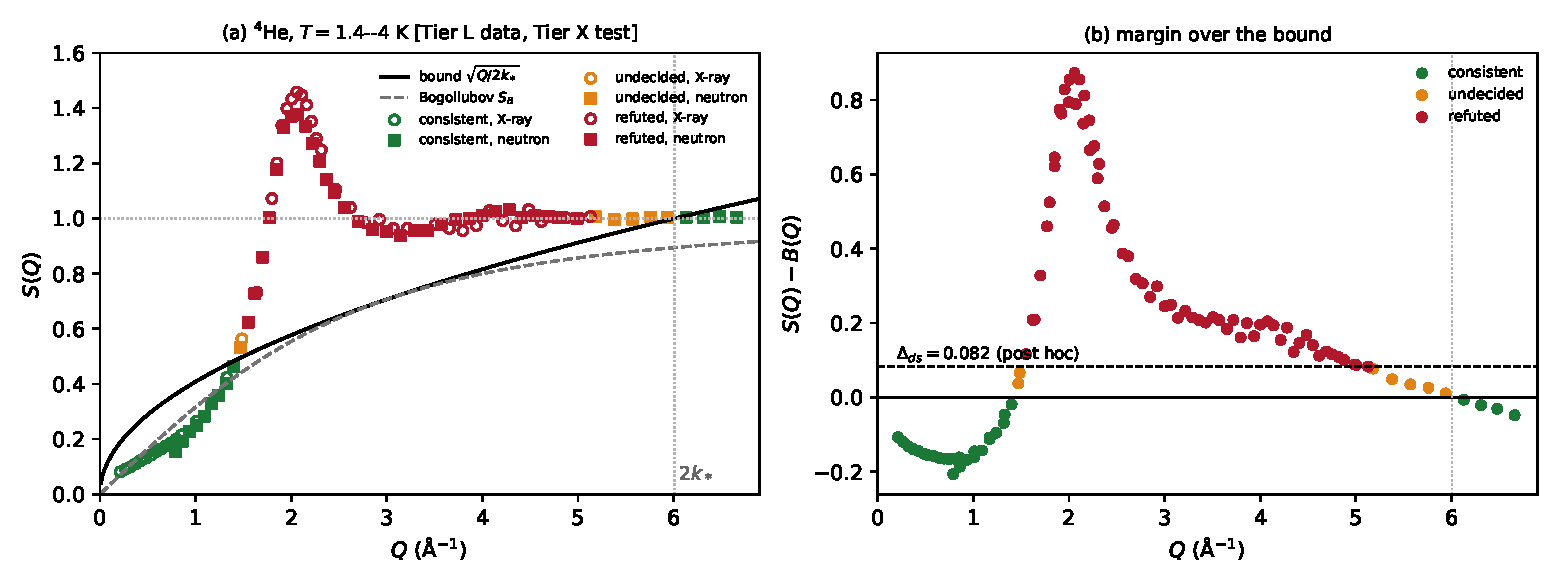
\includegraphics[width=\textwidth]{data/fig_he4.pdf}
\caption{$^4$He, Table~14.1 of~\cite{db}. (a) $S(Q)$ against $B(Q)=\sqrt{Q/2\ks}$ (black), the Bogoliubov $\SB$ with the $^4$He sound speed (dashed) and $S=1$ (dotted); open circles X-ray, filled squares neutron; colour is the verdict. (b) The margin
$S-B$ with $0$ and the post hoc $\Delta_{ds}$ marked. Data \tier{L}, evaluation \tier{X}. Generated by \texttt{make\_figures.py} from \texttt{data/test\_he4.csv}.}\label{fig:he}
\end{figure}

\paragraph{Result \tier{X, PH-X-0001}.} Of the $\PHNPoints$ points, $\PHNCons$ are consistent, $\PHNUnd$ undecided and $\PHNRef$ refuted ($\PHNRefXray$ X-ray, $\PHNRefNeutron$ neutron). The last consistent point is $Q=\PHLastConsQ$ ($S=\PHLastConsS$ against $B=\PHLastConsB$) and the first exceeding point is $Q=\PHFirstExQ$
($S=\PHFirstExS$ against $B=\PHFirstExB$), so the onset lies in $(\PHLastConsQ,\PHFirstExQ]$\,\AA$^{-1}$, i.e.\ $k/\ks\approx0.47$--$0.49$. The strict refuted run is contiguous from $Q=\PHStrictLo$ to $\PHStrictHi$\,\AA$^{-1}$; the nominal exceeding run extends to $Q=\PHNominalHi$, approaching $2\ks=\PHTwoKstar$,
where $B\to1$ and every $S\approx1$ passes vacuously. In the roton/peak region $1.7\le Q\le2.4$\,\AA$^{-1}$ all $\PHRotonN$ points are refuted, with $S/B$ between $\PHRotonRatioLo$ and $\PHRotonRatioHi$ and smallest margin $\PHRotonMinMargin$ ($S=\PHPeakS$ at $Q=\PHPeakQ$ against $B=\PHPeakBound$).
Beyond the peak ($3\lesssim Q\lesssim5.2$) $S\approx1$ against $B=0.71$--$0.93$: this is the same kind of failure as the free-particle control, not roton physics. Table~\ref{tab:reg} gives the breakdown.

\paragraph{Sensitivity to the post hoc threshold, and to the choice of dataset \tier{X, PH-X-0001}.} The counts depend on the third decimal of $\Delta_{ds}$ only at large $Q$: the points with margin between $0.07$ and $0.09$ are $Q=4.99$ ($0.0886$, neutron), $5.004$ ($0.0873$, X-ray), $5.129$ ($0.0830$, X-ray) and $5.18$ ($0.0774$, neutron). The endpoint $Q=\PHStrictHi$ of the strict run is therefore refuted by $0.0830$ against $\Delta_{ds}=\PHDeltaDS$, and $Q=5.18$ is undecided at $0.0774$.
Moving $\Delta_{ds}$ over $0.07$--$0.10$ changes the number refuted between $60$ and $64$ (of $99$), the number refuted above $2.4$\,\AA$^{-1}$ between $36$ and $40$, and the X-ray refuted count between $30$ and $32$, while the $29$ consistent points and the $21$ roton-region refutations do not change. So the strict-run endpoint, the region counts above $2.4$\,\AA$^{-1}$ and the X-ray refuted count ($\PHNRefXray$) should be read as threshold-dependent; the roton-region result is not: its smallest margin is $\PHRotonMinMargin$, about $4.0\,\Delta_{ds}$, and every roton point has margin $>0$.
Donnelly and Barenghi themselves recommend the X-ray data for $Q<1$\,\AA$^{-1}$ and the neutron data for $Q>1$\,\AA$^{-1}$~\cite{db}. This paper uses both sets throughout. On that recommended subset ($60$ points: $13$ X-ray with $Q<1$, $47$ neutron with $Q>1$) the verdicts at $\Delta_{ds}=\PHDeltaDS$ are $23$ consistent, $6$ undecided, $31$ refuted, and the roton/peak region holds $10$ neutron points, all refuted, with $S/B$ from $1.62$ to $2.38$ and the same smallest margin $\PHRotonMinMargin$, still refuted at $\Delta_{ds}=0$. The roton conclusion is unchanged. (Computed by \texttt{revision\_checks.py} from \texttt{data/test\_he4.csv}; output in \texttt{revision\_checks.json}.)

\begin{table}[t]\centering\small
\caption{$^4$He verdicts by region (\tier{X, PH-X-0001}); ratio is $S/B$. Regions are fixed by the verdict runs, not preregistered.}\label{tab:reg}
\begin{tabular}{lrrrrr}\toprule
$Q$ (\AA$^{-1}$) & points & consistent & undecided & refuted & $S/B$\\\midrule
\tabinput{gen/table_regions.tex}\bottomrule\end{tabular}
\end{table}

\paragraph{Controls \tier{X, PH-X-0002}.} \emph{Positive:} the homogeneous Bogoliubov $\SB$ at the same $\PHCtlBogN$ abscissae gives $\PHCtlBogViol$ violations (max $S/B=\PHCtlBogMax$). With Gaussian noise of $\sigma=0.01/0.02/0.04$ the fraction of 2000 trials producing any refuted point is $\PHFpOne/\PHFpTwo/\PHFpFour$, so the strict criterion has
essentially no false positives at the measured scatter ($\PHRmsSpline$), but it does at $0.04$. \emph{Negative:} $S\equiv1$ exceeds $B$ at $\PHCtlFreeNom$ points (exactly those with $Q<2\ks$; $\PHCtlFreeStrict$ strictly), and a planted $1.5\,\SB$ at $\PHCtlPlantNom$ ($\PHCtlPlantStrict$ strictly).
\emph{Transcription:} two independent parses of the HTML (regex over stripped text; an \texttt{html.parser} walk) give identical numbers ($\PHParseA$ for Table~14.1 and $\PHParseB$ for the spline table), with monotone $Q$ in both columns and spot checks against the printed page.
\emph{Self-consistency of the data \tier{X, PH-X-0003}:} Feynman's relation read as $S\le\eps_0/\eps$ with Godfrin's measured $\eps(k)$ holds at all but $\PHFeynExceed$ of $\PHFeynN$ points; the two exceptions, $Q=\PHFeynQa$ and $\PHFeynQb$, are both X-ray points at the lowest $Q$, consistent with (not proof of) thermal $S$ at $T\ge1.38$\,K. They are reported, not dropped.

\paragraph{Reading \tier{C, PH-C-0004}.} The comparison can be checked by hand at the peak, from the tabulated row and $\ks$ alone: at $Q=\PHPeakQ$\,\AA$^{-1}$ the table gives $S=\PHPeakS$ while $\sqrt{Q/2\ks}=\sqrt{\PHPeakQ/\PHTwoKstar}=\PHPeakBound$, so $S>\sqrt{Q/2\ks}+\Delta_{ds}$ with margin $\PHPeakS-\PHPeakBound\approx0.87$ (the neutron peak, $1.376$ at $Q=2.070$ against $0.587$, gives $0.79$). The tabulated $S(Q)$ exceeds the Bogoliubov envelope for $Q\gtrsim1.5$\,\AA$^{-1}$ and in the whole roton region by a factor $1.6$--$2.5$, far outside the $0.082$ spread between the two datasets and the $0.019$ scatter about the spline. Read through Steps~11 and~5, that says that the $^4$He liquid is not a Bogoliubov gas
with its own sound speed, which is the textbook fact that $k a\ll1$ fails in $^4$He. It is conditional on: the data being secondary; $T=1.4$--$4$\,K data standing for the $T\to0$ ground-state $S$ (the temperature dependence of the peak was not quantified, and no source for it was checked); and the post hoc $\Delta_{ds}$.
It does not use the Feynman--Bijl bound to bound anything about $^4$He, and nothing here refutes Bogoliubov theory in its range of validity.

\subsection{Trapped Bose gases}\label{sec:bec}
\paragraph{Comparator, fixed by a positive control \tier{X, PH-X-0004}.} A trapped cloud is not homogeneous, so the homogeneous bound of Step~11 cannot be applied with a single $\ks$. The LDA model of Step~12 was built with the Stamper-Kurn parameters ($q=\PBQ$\,$\mu\mathrm{m}^{-1}$ fixed by $\hb q^2/2m=h\times1.38$\,kHz, as in their Fig.~3 caption; Na-23
mass $22.98976928$\,u) and checked three ways: it reproduces the phonon closed form $\tfrac{15\pi}{32}\sqrt{\eps_0/2\mu}$ of \tier{L, PH-L-0001} to a relative \PBClosedA{} at $\eps_0/\mu=10^{-6}$ (\PBClosedB{} at $10^{-4}$, as expected of the next-order term); it reproduces the solid curve of their Fig.~3a read at six columns to $|\Delta S|\le\PBSolidMax$ (which also validates the $q$,
$\mu$ and mass inputs); and on $\PBNCurve$ values of $\mu/h$ between $0.5$ and $12$\,kHz the trapped model \emph{exceeds a single-$\ks$ bound} at $\PBPeakFail$ (peak $c=\sqrt{\mu/m}$), $\PBCeffFail$ ($c_{\rm eff}=0.68\sqrt{\mu/m}$) and $\PBMeanFail$ (mean-density $c$) points, and never ($\PBLdaFail$) exceeds the LDA-averaged bound $B_{\rm LDA}$
(Figure~\ref{fig:bec}b). On a $6\times7$ grid of $(\mu,q)$ for Rb there are $\PBGridViol$ violations of $S_{\rm LDA}\le B_{\rm LDA}$ out of $\PBGridN$, while $S=1$ exceeds it at $\PBGridFree$. Only $B_{\rm LDA}$ is therefore a valid comparator for a trapped gas: single-$\ks$ bounds fail their own positive control.

\begin{figure}[t]\centering
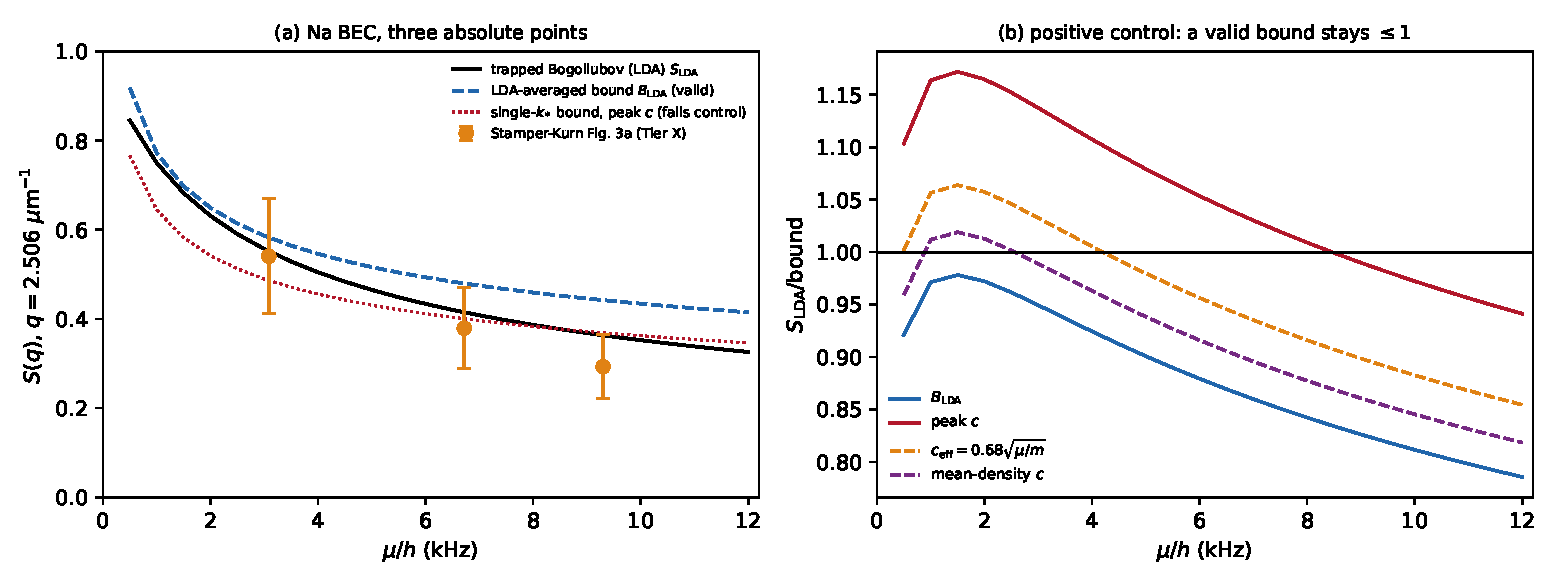
\includegraphics[width=\textwidth]{data/fig_bec.pdf}
\caption{Trapped Na condensate at fixed $q$ (\tier{X}). (a) Stamper-Kurn et al.\ Fig.~3a points read from the figure (error bars: half the plotted bar) against the LDA Bogoliubov model and two bounds. (b) Positive control: $S_{\rm LDA}$ divided by each candidate bound; a valid bound stays $\le1$.
Generated by \texttt{make\_figures.py}.}\label{fig:bec}
\end{figure}

\begin{table}[t]\centering\small
\caption{Stamper-Kurn et al.\ Fig.~3a (Na, $q=\PBQ$\,$\mu\mathrm{m}^{-1}$; values read from the figure, \tier{X, PH-X-0005}); $z=(S-B_{\rm LDA})/\sigma$; last column $S_{\rm LDA}/B_{\rm LDA}$.}\label{tab:sk}
\begin{tabular}{rrrrrrrr}\toprule
$n_{\rm pk}$ & $\mu/h$ (kHz) & $S$ & $\sigma$ & $S_{\rm LDA}$ & $B_{\rm LDA}$ & $z$ & model/bound\\\midrule
\tabinput{gen/table_sk.tex}\bottomrule\end{tabular}
\end{table}

\paragraph{Stamper-Kurn \tier{X, PH-X-0005}.} All three points lie below $B_{\rm LDA}$ (Table~\ref{tab:sk}): no refutation of trapped Bogoliubov. The test has little power: the model sits at $\PBSkRatioLo$--$\PBSkRatioHi$ of the bound ($B_{\rm LDA}=\PBSkBoundLo$--$\PBSkBoundHi$), and with $1\sigma$ bars of $0.07$--$0.13$ a refutation would need $S$
about one $\sigma$ above the bound. Three points read from a figure do not establish ``BEC consistent'', and that is not claimed.

\paragraph{Steinhauer \tier{X, PH-X-0006}.} The authors state that the plotted closed circles are the measured $S(k)$ \emph{multiplied by 2.3} to give rough agreement with the LDA Bogoliubov curve \tier{L, PH-L-0002}; a test on them is circular. Recorded for completeness: $\PBStNominal$ of $\PBStN$ exceed $B_{\rm LDA}$ nominally, none by more than $\PBStMaxZ\sigma$; un-rescaled, $\PBStRaw$ do, and the unresolved factor dominates. The open circles are $\eps_0/\omega$ from the measured
dispersion through Feynman's relation (Eq.~2 of their paper, from the f-sum rule), a re-expression of the spectrum and not a diffraction value; they follow the LDA model (rms difference $\PBStOpenRms$, max $\PBStOpenMax$). Not decisive either way. The same rescaling habit occurs in a phonon-imprinting experiment (Shammass et al.~\cite{sham}, a factor $1.5$);
only Stamper-Kurn's ratio is absolute.

%% =====================================================================================================================
\section{rusty-SUNDIALS and LeanFlow: no change in this lane}\label{sec:rusty}
The request for this programme was to improve rusty-SUNDIALS or LeanFlow along the way. In lane P6 \textbf{no change was made to either}: no commit exists, so none is cited. The numerics of Section~\ref{sec:data} are Python/numpy/scipy scripts (Tier~X); the Lean compiles use the programme's
\texttt{lean\_pinned.py} driver unchanged. The Gross--Pitaevskii linear-response check in rusty-SUNDIALS that accompanies the earlier Bogoliubov preprint~\cite{bsk} was not repeated or extended here. A natural follow-up that would use the solver is a CVODE time-domain GP calculation of $S(q)$ in the trap, to replace the LDA by a direct
computation and remove the figure-read comparison; it was not attempted.

%% =====================================================================================================================
\section{Claim ledger}\label{sec:ledger}
\texttt{ledger/build\_ledger.py} files \PLedN{} claims: \PLedA{} at Tier~A, \PLedL{} at L, \PLedC{} at C and \PLedX{} at X. Each has a content-addressed evidence blob in \texttt{ledger/evidence/}: verbatim axiom lines and source hashes (A), excerpts in \texttt{ledger/sources/excerpts.json} (L; prose as extracted, mathematics transcribed linearly), the argument text (C), and result files with \texttt{claim\_licence: false} (X).
The gate enforces a closure rule: a claim cannot be filed above the effective tier of anything it rests on. For that reason the physical gloss of the He-4 result (\texttt{PH-C-0004}) rests on A and L rows only, and the arithmetic it glosses is the separate Tier~X row \texttt{PH-X-0001}. The Elenchus gate
(\texttt{tools/ledger.py ledger.json -{}-evidence-dir evidence}, output in \texttt{ledger/gate\_output.txt}) exits with code~\PGateExit. It reports \textbf{\PGateBlock{} blocking findings} and \textbf{\PGateFlag{} flags}, all \texttt{LEDGER\_UNAUDITED\_TIER\_A}, one for each Tier~A row: no person has certified that the statements mean what their glosses say. The flags remain open.
The L excerpts are prose, not theorem statements, so the citation gate (\texttt{citation\_check.py}) was not run on them.

%% =====================================================================================================================
\section{Limitations}\label{sec:lim}
\begin{itemize}
\item \textbf{Verification status.} The Lean module was compiled by its producer and recompiled once by the same pipeline; it was then independently recompiled by a separate AI auditor with a private olean build (same axiom lines, same file hashes, planted controls and two auditor mutations caught). No human has audited the Lean statements or the hand proofs, every Tier~A ledger row still has \texttt{audit: null}, and the Elenchus \texttt{elenchus\_check.py} could not be used by the auditor (it does not see Mathlib), so the equivalent check was the pinned-toolchain \lean{\#print axioms} audit. The Bogoliubov envelope used in the test was also independently recompiled in its original cross-stack form~\cite{bsk}.
\item \textbf{The physics is not in Lean.} The f-sum value, the symmetry, the ground-state property of the physical fluid and momentum conservation are hypotheses or \tier{C}; the abstract finite-dimensional $H$ is not the Bogoliubov Hamiltonian, so ``the Bogoliubov ground state saturates the operator bound'' is \tier{C/L}.
\item \textbf{Reading a measured $S$ as a bound on $\eps$} needs the $T=0$ ground-state $S$. The $^4$He data are at $1.4$--$4$\,K, include thermal $S$ (two X-ray points already exceed the Feynman self-check), and the temperature dependence of the roton peak was not quantified.
\item \textbf{Data.} $^4$He values are secondary (web edition of a compilation, assumed to reproduce the 1998 table; primary tables unseen) with no uncertainties; $\Delta_{ds}$ is a post hoc proxy outside the preregistration; the Table~14.1 year for Svensson is misprinted in the compilation and corrected from~\cite{mg}. All Bose-gas values are read from figures (\tier{X}), three absolute points exist, and Steinhauer's carries an unexplained factor 2.3.
\item \textbf{Test power and novelty.} The envelope is an upper bound, so the test can refute but never confirm; the $^4$He outcome is a textbook fact; the Feynman--Bijl formalisation is a textbook argument.
\item \textbf{Not read.} Feynman (1954), Bijl (1940), Bogoliubov (1947), the primary $^4$He papers and the 1998 journal table were not read by us; they are cited only as given by the sources that were read.
\item \textbf{Rusty/LeanFlow.} No improvement was made (Section~\ref{sec:rusty}).
\end{itemize}

%% =====================================================================================================================
\section{Reproducibility}\label{sec:repro}
AutoevolveAI files are uncommitted on top of base \texttt{9d245742c1655852103abb28f585e21af54851e6} (branch \texttt{worktree-openai-math-discovery}). Lean source sha256 values (they \PLShaMatch{} the values recorded at stage WORK2):
\begin{itemize}\scriptsize
\item \texttt{Basic.lean}: \texttt{\PLShaBasic}
\item \texttt{NegativeControls.lean}: \texttt{\PLShaNeg}
\item \texttt{PositiveControls.lean}: \texttt{\PLShaPos}
\item \texttt{Controls.lean}: \texttt{\PLShaCtl}
\end{itemize}
Paper-stage rerun of the four compiles by the same AI pipeline (\tier{X, PH-X-0008}; not itself an independent check): \PLRerun. The independent recompile by the separate AI auditor (private olean directory; its scripts and outputs are listed in \texttt{AUDIT.md}) gave rc~0 for all four files, sha256 values equal to those above, 21/21, 4/4 and 3/3 \lean{\#print axioms} lines each exactly \lean{[propext, Classical.choice, Quot.sound]}, and exposed both planted cheats and both of its own mutations. Commands, from the worktree root:
\begin{lstlisting}[basicstyle=\ttfamily\tiny]
taskset -c 4-7 python3 scripts/certified_numerics/lean_pinned.py compile formal_cert/Programmes/FeynmanBijl/Basic.lean --olean Programmes.FeynmanBijl.Basic --json-out <out>.json
taskset -c 4-7 python3 scripts/certified_numerics/lean_pinned.py compile formal_cert/Programmes/FeynmanBijl/NegativeControls.lean --olean Programmes.FeynmanBijl.NegativeControls --json-out <out>.json
taskset -c 4-7 python3 scripts/certified_numerics/lean_pinned.py compile formal_cert/Programmes/FeynmanBijl/PositiveControls.lean --json-out <out>.json
taskset -c 4-7 python3 scripts/certified_numerics/lean_pinned.py compile formal_cert/Programmes/FeynmanBijl/Controls.lean --json-out <out>.json
python -I results/programmes/2026-10-25/P6/scripts/axiom_gate.py ; python -I results/programmes/2026-10-25/P6/scripts/analysis.py   # He-4 and BEC analysis -> results.json
python -I papers/prog_superfluid_structure_factor/rerun_lean.py      # paper-stage rerun
python -I papers/prog_superfluid_structure_factor/gen_inputs.py ; python -I papers/prog_superfluid_structure_factor/make_figures.py
python -I papers/prog_superfluid_structure_factor/ledger/build_ledger.py ; python -I papers/prog_superfluid_structure_factor/ledger/run_gate.py
python -I papers/prog_superfluid_structure_factor/revision_checks.py   # threshold sensitivity, recommended subset -> revision_checks.json
python -I papers/prog_superfluid_structure_factor/build_pdf.py        # clean build, pdflatex three times
\end{lstlisting}
The Python is the programme's virtual environment (numpy, scipy, matplotlib). Inputs and outputs of the analysis are copied into \texttt{data/} (\texttt{test\_he4.csv}, the Table~14.1 parse, the digitised BEC values, \texttt{results.json}, the scripts). The Donnelly--Barenghi page (sha256 \texttt{b5a3bc07\ldots 2f304b8}, downloaded 2026-10-25) is kept outside the repository; only the extracted numbers
are in the record. The excerpts of the alphaXiv-read papers are in \texttt{ledger/sources/excerpts.json}: prose as extracted, mathematics transcribed linearly (for instance $\pm\to$ \texttt{+-}, $\mu\to$ \texttt{mu}, the square-root sign dropped), so a character-level match against the PDFs fails for most fragments that contain mathematics.

\begin{thebibliography}{99}\small
\bibitem{bsk} X.~Callens, \emph{The Bogoliubov structure factor under the dual-scale envelope $\sqrt{k/2k_*}$: kernel-checked shape theorems, a one-sided diffraction test, and a Gross--Pitaevskii linear-response check in rusty-SUNDIALS}, preprint v1, doi:10.5281/zenodo.23646117 (2026; DOI reserved on Zenodo, publication status not checked here).
\bibitem{ar} X.~Callens, four companion preprints of the same autoresearch round: bilayer dipolar excitons doi:10.5281/zenodo.23646103; planar Yukawa doi:10.5281/zenodo.23646105; Rytova--Keldysh doi:10.5281/zenodo.23646107; $\sigma=3$ dyadic enstrophy doi:10.5281/zenodo.23646111 (2026; DOIs reserved, publication status not checked here). The tier conventions of this preprint follow them.
\bibitem{txt} X.~Callens, \emph{The Triangular Lattice and Universal Optimality} (textbook), doi:10.5281/zenodo.23295142 (2026).
\bibitem{sk} D.~M. Stamper-Kurn, A.~P. Chikkatur, A.~G\"orlitz, S.~Inouye, S.~Gupta, D.~E. Pritchard, W.~Ketterle, \emph{Excitation of phonons in a Bose-Einstein condensate by light scattering}, Phys.\ Rev.\ Lett.\ \textbf{83}, 2876 (1999), arXiv:cond-mat/9906035v2 (read: pp.~1--4, Fig.~3, Eq.~3, Eq.~5).
\bibitem{st} J.~Steinhauer, R.~Ozeri, N.~Katz, N.~Davidson, \emph{Excitation spectrum of a Bose-Einstein condensate}, Phys.\ Rev.\ Lett.\ \textbf{88}, 120407 (2002), arXiv:cond-mat/0111438v1 (read: pp.~1--5; the journal reference is confirmed as ref.~[4] of Shammass et al.~\cite{sham}, not checked against the journal itself).
\bibitem{godfrin} H.~Godfrin, K.~Beauvois, A.~Sultan, E.~Krotscheck, J.~Dawidowski, B.~F{\aa}k, J.~Ollivier, \emph{The dispersion relation of Landau elementary excitations and the thermodynamic properties of superfluid $^4$He}, arXiv:2012.09067v1 (2020) (read: alphaXiv text extraction; $c$ and $m_4$).
\bibitem{mg} T.~Morresi, G.~Garberoglio, \emph{Revisiting the properties of superfluid and normal liquid $^4$He using ab initio potentials}, arXiv:2501.08730v1 (2025) (read: Fig.~2 caption, ref.~[50]).
\bibitem{db} R.~J. Donnelly, C.~F. Barenghi, \emph{The observed properties of liquid helium at the saturated vapor pressure}, J.\ Phys.\ Chem.\ Ref.\ Data \textbf{27}, 1217 (1998); web edition ch.~14, \url{https://pages.uoregon.edu/rjd/vapor15.htm} (read: the web edition; the journal edition was not seen).
\bibitem{sham} I.~Shammass, S.~Rinott, A.~Berkovitz, R.~Schley, J.~Steinhauer, \emph{The phonon dispersion relation of a Bose-Einstein condensate}, arXiv:1207.3440 (v2 read on alphaXiv; excerpt on the amplitude factor 1.5).
\bibitem{feyn} R.~P. Feynman, Phys.\ Rev.\ \textbf{94}, 262 (1954); cited as given in~\cite{st} (ref.~[11]), \emph{not read by us}.
\bibitem{bijl} A.~Bijl, Physica \textbf{7}, 869 (1940); as cited in the lane record, \emph{not read by us}.
\bibitem{bog} N.~N. Bogoliubov, J.\ Phys.\ (USSR) \textbf{11}, 23 (1947); cited as given in~\cite{sk,st}, \emph{not read by us}.
\bibitem{rh} H.~N. Robkoff, R.~B. Hallock, Phys.\ Rev.\ B \textbf{24}, 159 (1981) and E.~C. Svensson, V.~F. Sears, A.~D.~B. Woods, P.~Martel, Phys.\ Rev.\ B \textbf{21}, 3638 (1980); cited as given in~\cite{db,mg}, \emph{not read by us}.
\bibitem{oai} OpenAI, openai/math release, \url{https://github.com/openai/math/tree/fd4aeeb2ee4fc729c18d98444fed42fd0529eeeb} (2026); used here only for its pinned Lean 4.34.1 + Mathlib build environment. AI-generated; not peer reviewed.
\end{thebibliography}
\end{document}
